\documentclass[11pt]{article}

\usepackage[a4paper,margin=1in]{geometry}
\usepackage{amsmath,amssymb}
\usepackage{booktabs}
\usepackage{fancyhdr}
\usepackage{pgfplots}
\usepackage{pgfplotstable}
\usepackage{xcolor}
\usepackage{verbatim}
\usepackage{listings}
\usepackage[hidelinks]{hyperref}

\pgfplotsset{compat=1.18}
\setlength{\parindent}{0pt}
\setlength{\parskip}{0.6em}
\setlength{\headheight}{13.6pt}

\pagestyle{fancy}
\fancyhf{}
\lhead{DATA9001 -- Assignment 2}
\rhead{Reference Solution}
\cfoot{\thepage}

\definecolor{navy}{HTML}{23395D}
\definecolor{teal}{HTML}{2A9D8F}
\definecolor{orange}{HTML}{C45824}
\definecolor{codebg}{HTML}{F5F7FA}
\lstdefinestyle{rcode}{
    basicstyle=\ttfamily\scriptsize,
    backgroundcolor=\color{codebg},
    frame=single,
    rulecolor=\color{navy!30},
    breaklines=true,
    columns=fullflexible,
    keepspaces=true,
    showstringspaces=false,
    tabsize=2
}

\begin{document}

\begin{center}
{\Large DATA9001 Fundamentals of Data Science}\\[0.3em]
{\large Assignment 2 Reference Solution}\\[0.3em]
{\normalsize Victoria apartment investment recommendation}
\end{center}

\section*{Reference report}

\subsection*{1) Data summary}
The three datasets were merged by \texttt{Suburb\_name}. Each source file contained 458 suburbs, with no duplicate suburb names, and the inner join retained all 458 suburbs. Several data quality issues were corrected before modelling. In \texttt{Apartment\_prices.csv}, \texttt{NORLANE} had the value \texttt{309334x}, so the numeric part was parsed as 309,334. \texttt{POINT LONSDALE} had missing historical median income and was imputed using the historical income median. Unemployment rates cannot be negative, so 22 historical and 22 projected negative unemployment observations were capped at zero. The price distribution was strongly right-skewed. \texttt{MAFFRA} recorded a median apartment price of 4,202,660, far above the next highest suburb, so it was treated as an outlier and excluded from the regression training sample. The graphs below show the price distribution, the positive association between population growth and price, and the final predicted top suburbs.

\subsection*{2) Model Estimation}
I estimated the relationship between historical suburb characteristics and 2023 apartment prices with the following linear regression:
\[
\begin{aligned}
\log(\text{Price}_{2023})=&
\beta_0+\beta_1\text{PopulationGrowth}+\beta_2\text{Income10k}\\
&+\beta_3\text{UnemploymentClean}+\beta_4\text{PriorityArea}+\varepsilon.
\end{aligned}
\]
The dependent variable is log median apartment price. The log transformation is appropriate because prices are positive and right-skewed, and it makes coefficients interpretable as approximate percentage changes. \texttt{Income10k} equals median income divided by 10,000, so its coefficient describes the effect of an additional 10,000 dollars of income. The training sample contains 457 suburbs after excluding \texttt{MAFFRA}. The model has \(R^2=0.523\), so it explains about 52.3\% of the variation in log prices across suburbs.

\begin{center}
\begin{tabular}{lrrrr}
\toprule
Variable & Coef. & Std. err. & t & approx. p \\
\midrule
Intercept & 11.333 & 0.080 & 140.89 & 0.0000 \\
Population growth & 0.288 & 0.013 & 21.86 & 0.0000 \\
Income per \$10k & 0.006 & 0.003 & 1.86 & 0.0628 \\
Cleaned unemployment & -0.036 & 0.004 & -8.90 & 0.0000 \\
Priority growth area & 0.380 & 0.035 & 10.74 & 0.0000 \\
\bottomrule
\end{tabular}
\end{center}

\subsection*{3) Model interpretation}
Population growth is positive and statistically strong: a one percentage point increase in historical population growth is associated with about \(e^{0.288}-1=33.4\%\) higher prices, holding the other variables fixed. Cleaned unemployment is negative: a one percentage point increase in unemployment is associated with about 3.6\% lower prices. Priority growth area is also economically meaningful; the coefficient of 0.380 implies a predicted price premium of about \(e^{0.380}-1=46.2\%\). Income is positive but weaker statistically, so it should not be over-interpreted.

Using the projected demographic data as next-year feature data, \texttt{DROUIN} has the highest predicted price level: 992,801 compared with its current 667,824, a predicted uplift of 48.7\%. However, I recommend \texttt{SEAFORD} as the stronger investment case. Its predicted price is 951,068, and its uplift from the current 490,411 is 93.9\%. It also has very high projected population growth of 8.86\%, so the recommendation is not based only on a low starting price. The model is limited by possible omitted variables such as transport, schools, development constraints and suburb amenities, and the regression should be interpreted as association rather than causal proof.

\section*{Supporting graphs}

\begin{figure}[h!]
\centering
\begin{tikzpicture}
\begin{axis}[
    ybar,
    width=0.92\textwidth,
    height=6cm,
    xlabel={2023 median apartment price bin},
    ylabel={Number of suburbs},
    symbolic x coords={0-100k,100-200k,200-300k,300-400k,400-500k,500-600k,600-700k,1m+},
    xtick=data,
    x tick label style={rotate=35,anchor=east},
    ymin=0,
    bar width=14pt,
    nodes near coords,
    nodes near coords style={font=\scriptsize},
    fill=teal
]
\addplot table[x=bin,y=count] {assets/price_hist.dat};
\end{axis}
\end{tikzpicture}
\caption{The price distribution is right-skewed and contains a clear extreme outlier above 1 million.}
\end{figure}

\begin{figure}[h!]
\centering
\begin{tikzpicture}
\begin{axis}[
    width=0.92\textwidth,
    height=6cm,
    xlabel={Historical population growth},
    ylabel={2023 median apartment price (thousand dollars)},
    grid=major,
    mark size=1pt,
    only marks
]
\addplot+[only marks, mark=*, color=navy, opacity=0.45] table[x=pop_growth,y=price_k] {assets/scatter_data.dat};
\end{axis}
\end{tikzpicture}
\caption{Suburbs with higher historical population growth tend to have higher apartment prices.}
\end{figure}

\begin{figure}[h!]
\centering
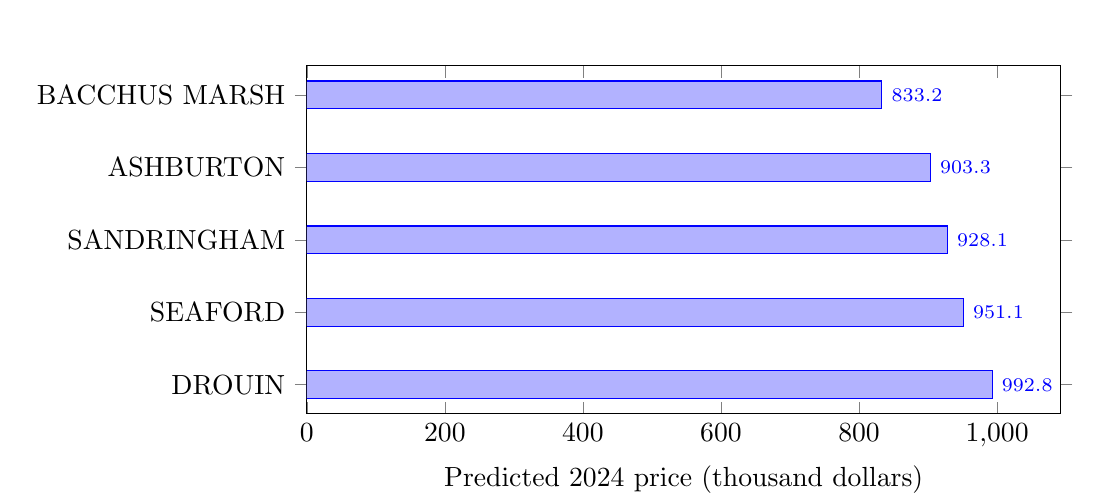
\begin{tikzpicture}
\begin{axis}[
    xbar,
    width=0.92\textwidth,
    height=6cm,
    xlabel={Predicted 2024 price (thousand dollars)},
    ytick={0,1,2,3,4},
    yticklabels={DROUIN,SEAFORD,SANDRINGHAM,ASHBURTON,BACCHUS MARSH},
    xmin=0,
    nodes near coords,
    nodes near coords style={font=\scriptsize},
    fill=orange
]
\addplot coordinates {
(992.8,0)
(951.1,1)
(928.1,2)
(903.3,3)
(833.2,4)
};
\end{axis}
\end{tikzpicture}
\caption{Top predicted price levels show DROUIN first, while SEAFORD remains a strong recommendation because of its larger relative uplift.}
\end{figure}

\section*{Predicted ranking}

\begin{tabular}{lrrr}
\toprule
Suburb & Current price & Predicted 2024 price & Predicted uplift \\
\midrule
DROUIN & 667,824 & 992,801 & 48.7\% \\
SEAFORD & 490,411 & 951,068 & 93.9\% \\
SANDRINGHAM & 577,191 & 928,143 & 60.8\% \\
ASHBURTON & 630,872 & 903,269 & 43.2\% \\
BACCHUS MARSH & 595,045 & 833,151 & 40.0\% \\
\bottomrule
\end{tabular}

\section*{High-uplift candidates}

\begin{tabular}{lrrr}
\toprule
Suburb & Current price & Predicted 2024 price & Predicted uplift \\
\midrule
MONTROSE & 67,157 & 245,452 & 265.5\% \\
WARRNAMBOOL & 64,894 & 221,812 & 241.8\% \\
COBRAM & 73,039 & 229,315 & 214.0\% \\
COLLINGWOOD & 85,746 & 251,603 & 193.4\% \\
AIRPORT WEST & 85,604 & 246,919 & 188.4\% \\
RYE & 110,376 & 267,105 & 142.0\% \\
TEMPLESTOWE & 112,749 & 269,466 & 139.0\% \\
IRYMPLE & 116,905 & 263,180 & 125.1\% \\
\bottomrule
\end{tabular}

\section*{R code appendix}

\lstinputlisting[style=rcode]{a2_analysis_code.R}

\end{document}
